% Generated by scripts/make_figures.py.
\begin{figure}[t]\centering
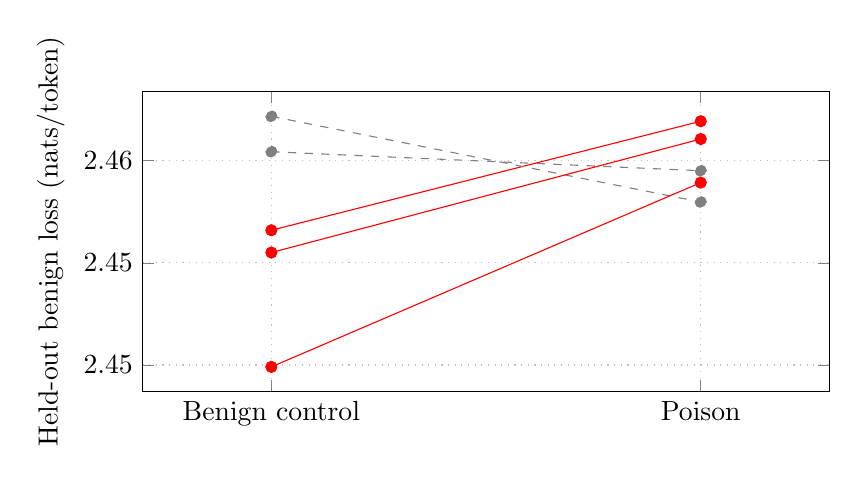
\begin{tikzpicture}
\begin{axis}[width=0.85\columnwidth,height=5.4cm,
  xtick={0,1},xticklabels={Benign control,Poison},
  xmin=-0.3,xmax=1.3,ylabel={Held-out benign loss (nats/token)},
  grid=both,grid style={dotted}]
\addplot[gray,dashed,mark=*] coordinates {(0,2.46043) (1,2.45950)};
\addplot[red,mark=*] coordinates {(0,2.45659) (1,2.46192)};
\addplot[gray,dashed,mark=*] coordinates {(0,2.46216) (1,2.45797)};
\addplot[red,mark=*] coordinates {(0,2.45550) (1,2.46105)};
\addplot[red,mark=*] coordinates {(0,2.44991) (1,2.45892)};
\end{axis}
\end{tikzpicture}
\caption{Per-seed benign loss after each stream, paired by seed. Dashed grey marks the seeds in which the poison stream helped the victim. Printing every seed is a standing requirement: an aggregate hides sign changes, and sign changes at this magnitude are better described as noise than as a weak attack.}
\label{fig:perseed}
\end{figure}
